\documentclass[letterpaper,12pt]{article}
\usepackage{tabularx} % extra features for tabular environment
\usepackage{amsmath}  % improve math presentation
\usepackage{amsfonts}
\usepackage{amssymb}
\usepackage{mathtools}
\usepackage{graphicx} % takes care of graphic including machinery
\usepackage[margin=1in,letterpaper]{geometry} % decreases margins
\usepackage{cite} % takes care of citations
\usepackage[final]{hyperref} % adds hyper links inside the generated pdf file
\usepackage{placeins}
\hypersetup{
	colorlinks=true,       % false: boxed links; true: colored links
	linkcolor=blue,        % color of internal links
	citecolor=blue,        % color of links to bibliography
	filecolor=magenta,     % color of file links
	urlcolor=blue         
}
\usepackage{blindtext}
%++++++++++++++++++++++++++++++++++++++++


\begin{document}

\title{ \textbf{Project 1: Thermal Storage Design\\
with PINNs}}
\author{A. Umeri}
\date{\today}
\maketitle

\begin{abstract}
The main objective of the project is to apply \textit{Physics Informed Neural Networks} (PINNs) to solve tasks
related to the preliminary design of a \textit{thermal energy storage}.
\end{abstract}
 

\section*{Task 1: PINNs for solving PDEs}
We consider the following system of \textit{reaction-convection-diffusion} equations:
\begin{align*}
\frac{\partial \bar{T}_{f}}{\partial t}+U_{f} \frac{\partial \bar{T}_{f}}{\partial x}=\alpha_{f} \frac{\partial^{2} \bar{T}_{f}}{\partial x^{2}}-h_{f}\left(\bar{T}_{f}-\bar{T}_{s}\right) \quad x \in[0,1],\: t \in[0,1] \\
\frac{\partial \bar{T}_{s}}{\partial t}=\alpha_{s} \frac{\partial^{2} \bar{T}_{s}}{\partial x^{2}}+h_{s}\left(\bar{T}_{f}-\bar{T}_{s}\right) \quad x \in[0,1],\: t \in[0,1] \tag{7}
\end{align*}

with the following initial and boundary conditions:
\begin{align*}
\bar{T}_{f}(x, t=0) & =\bar{T}_{s}(x, t=0)=T_{0}, & x \in[0,1] \\
\left.\frac{\partial \bar{T}_{s}}{\partial x}\right|_{x=0} & =\left.\frac{\partial \bar{T}_{s}}{\partial x}\right|_{x=1}=\left.\frac{\partial \bar{T}_{f}}{\partial x}\right|_{x=1}=0, & t \in[0,1]  \tag{8}\\
\bar{T}_{f}(x=0, t) & =\frac{T_{h o t}-T_{0}}{1+\exp (-200(t-0.25))}+T_{0}, & t \in[0,1] 
\end{align*}

and with the following constants:
\[
\begin{array}{rrrr}
\alpha_{f}=0.05, & h_{f}=5, & T_{h o t}=4, & U_{f}=1,  \tag{9}\\
\alpha_{s}=0.08, & h_{s}=,6 & T_{0}=1. &
\end{array}
\]

We approximate the solution of the system of PDEs with a \textit{physics informed neural network}. To this end we used a two-outputs neural network 
\[
N\!N_{\theta}\colon(t, x)\mapsto\left(\bar{T}_{f}^{\theta}, \bar{T}_{s}^{\theta}\right)
\]
with trainable parameters $\theta.$ For performance reasons we did not consider to implement two separate neural networks. We use the  \textit{PINNs tutorial} as foundation for our implementation. The following procedures have been suitably adapted to perform this task:
\begin{enumerate}
	\setlength\itemsep{-0.2em}
  	\item\textit{initial\_condition}
	\item\textit{add\_temporal\_boundary\_points}
	\item\textit{add\_spatial\_boundary\_points}
	\item\textit{add\_interior\_points}
	\item\textit{apply\_boundary\_conditions}
	\item\textit{compute\_pde\_residual}
	\item\textit{compute\_loss}
\end{enumerate}
The loss function takes into account the squared approximation error ($L_2$-norm of the residuals) at the temporal and spatial boundaries and interior points. 

Here are the approximations $(\bar{T}_{f}^{\theta}, \bar{T}_{s}^{\theta})$ given Sobol points as input:
\begin{figure}[!htb]
    \centering
    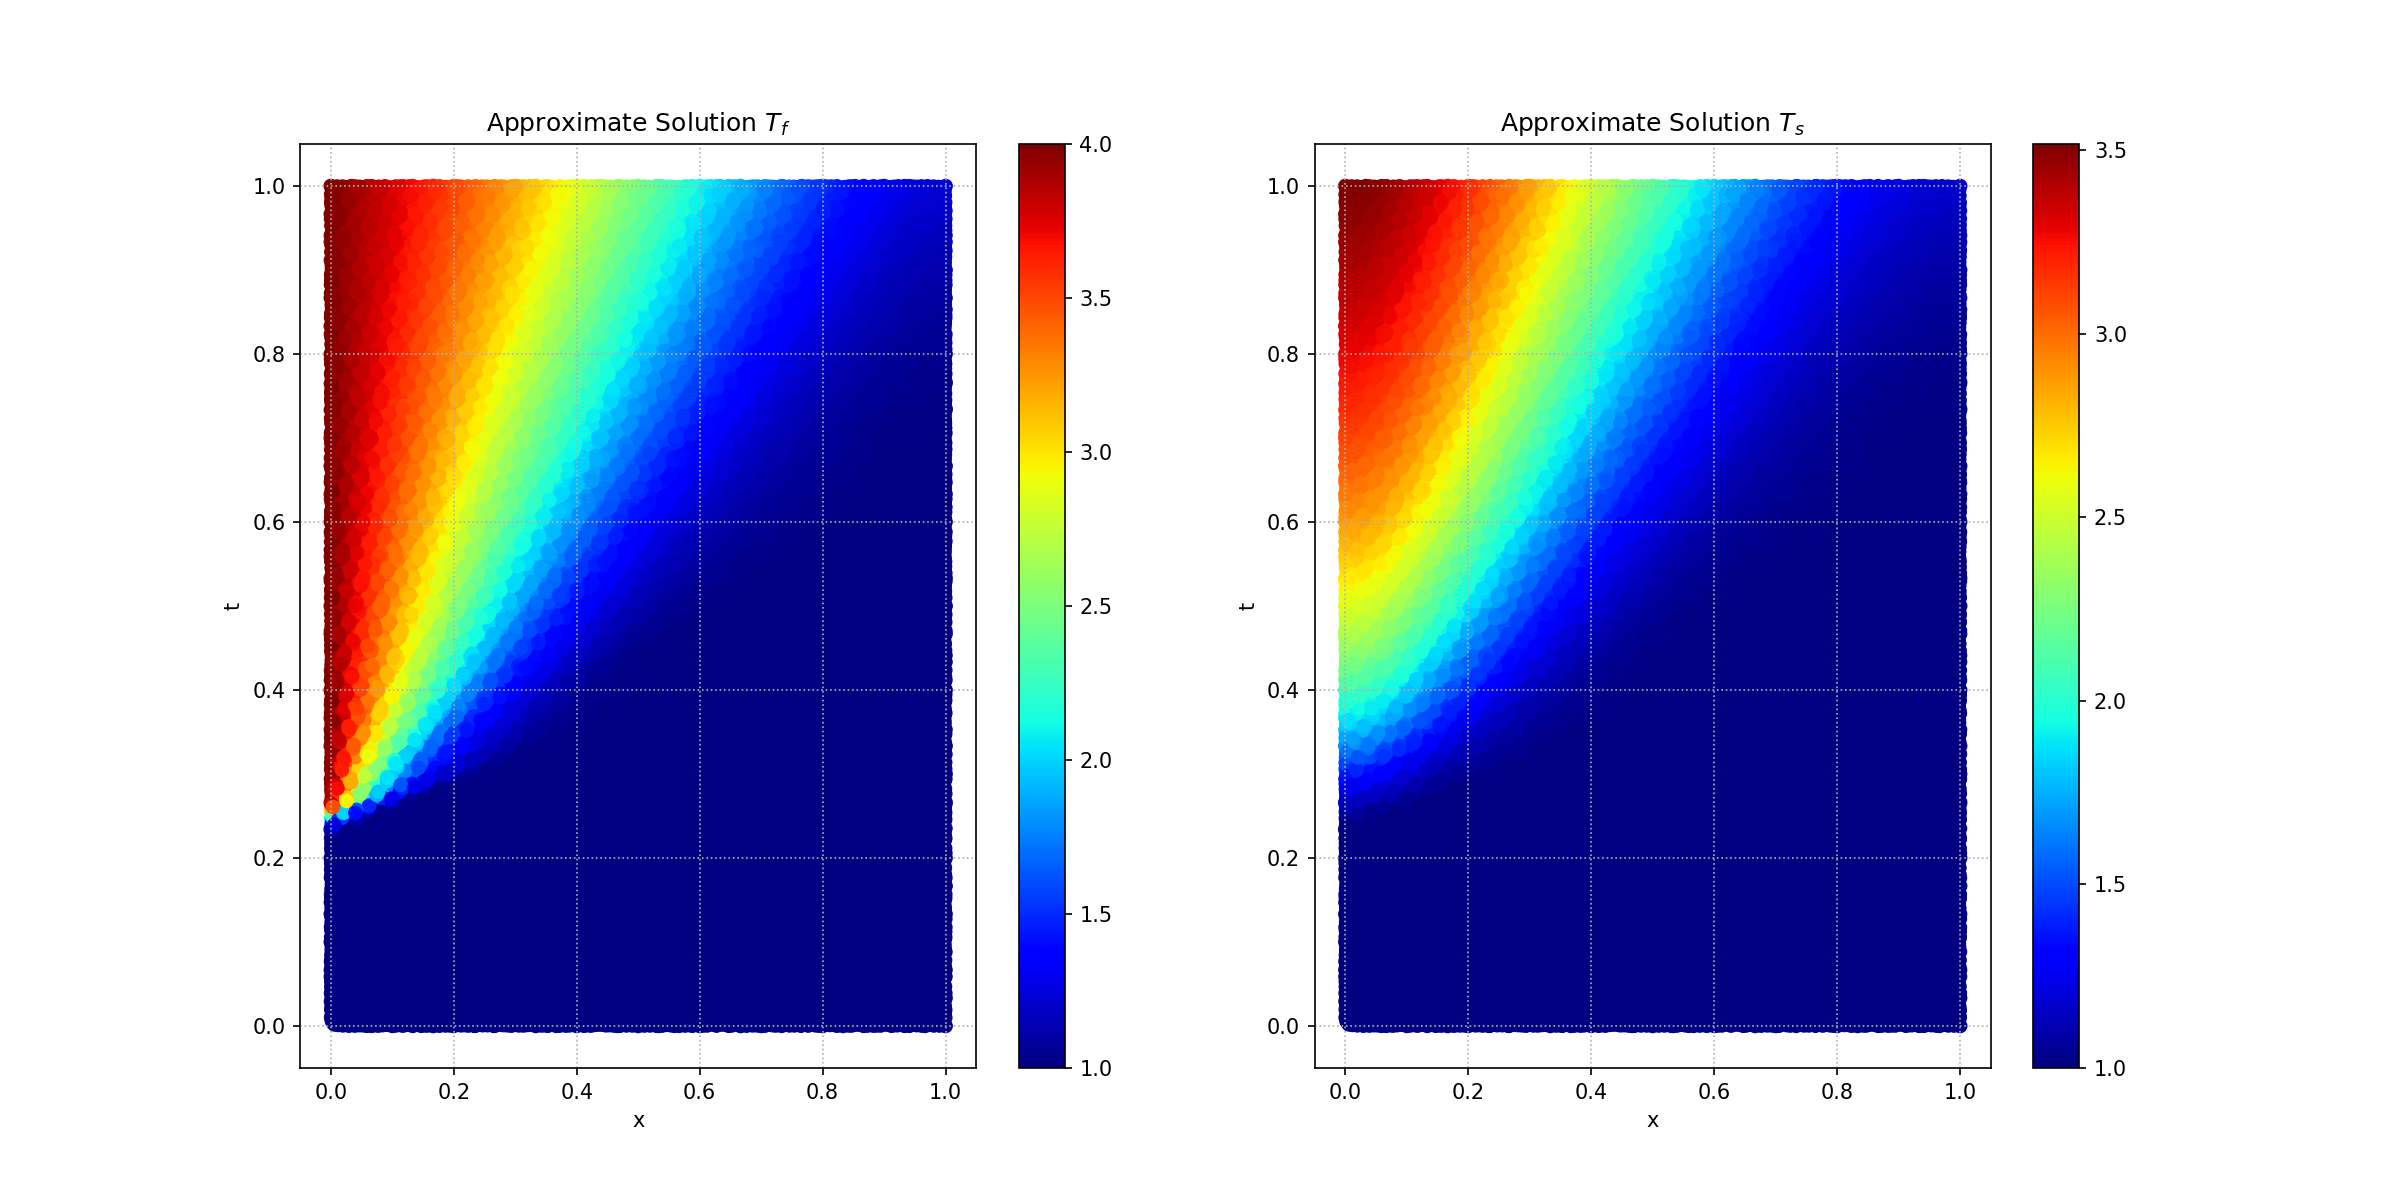
\includegraphics[width=.7\textwidth]{Graphics/Task1_Approximate_Solution.png}
    \caption{PINN-approximations $(\bar{T}_{f}^{\theta}, \bar{T}_{s}^{\theta})$ given Sobol points as input data.}
\end{figure}

Predictions have been made based on test data as well: 
\begin{figure}[!htb]
    \centering
    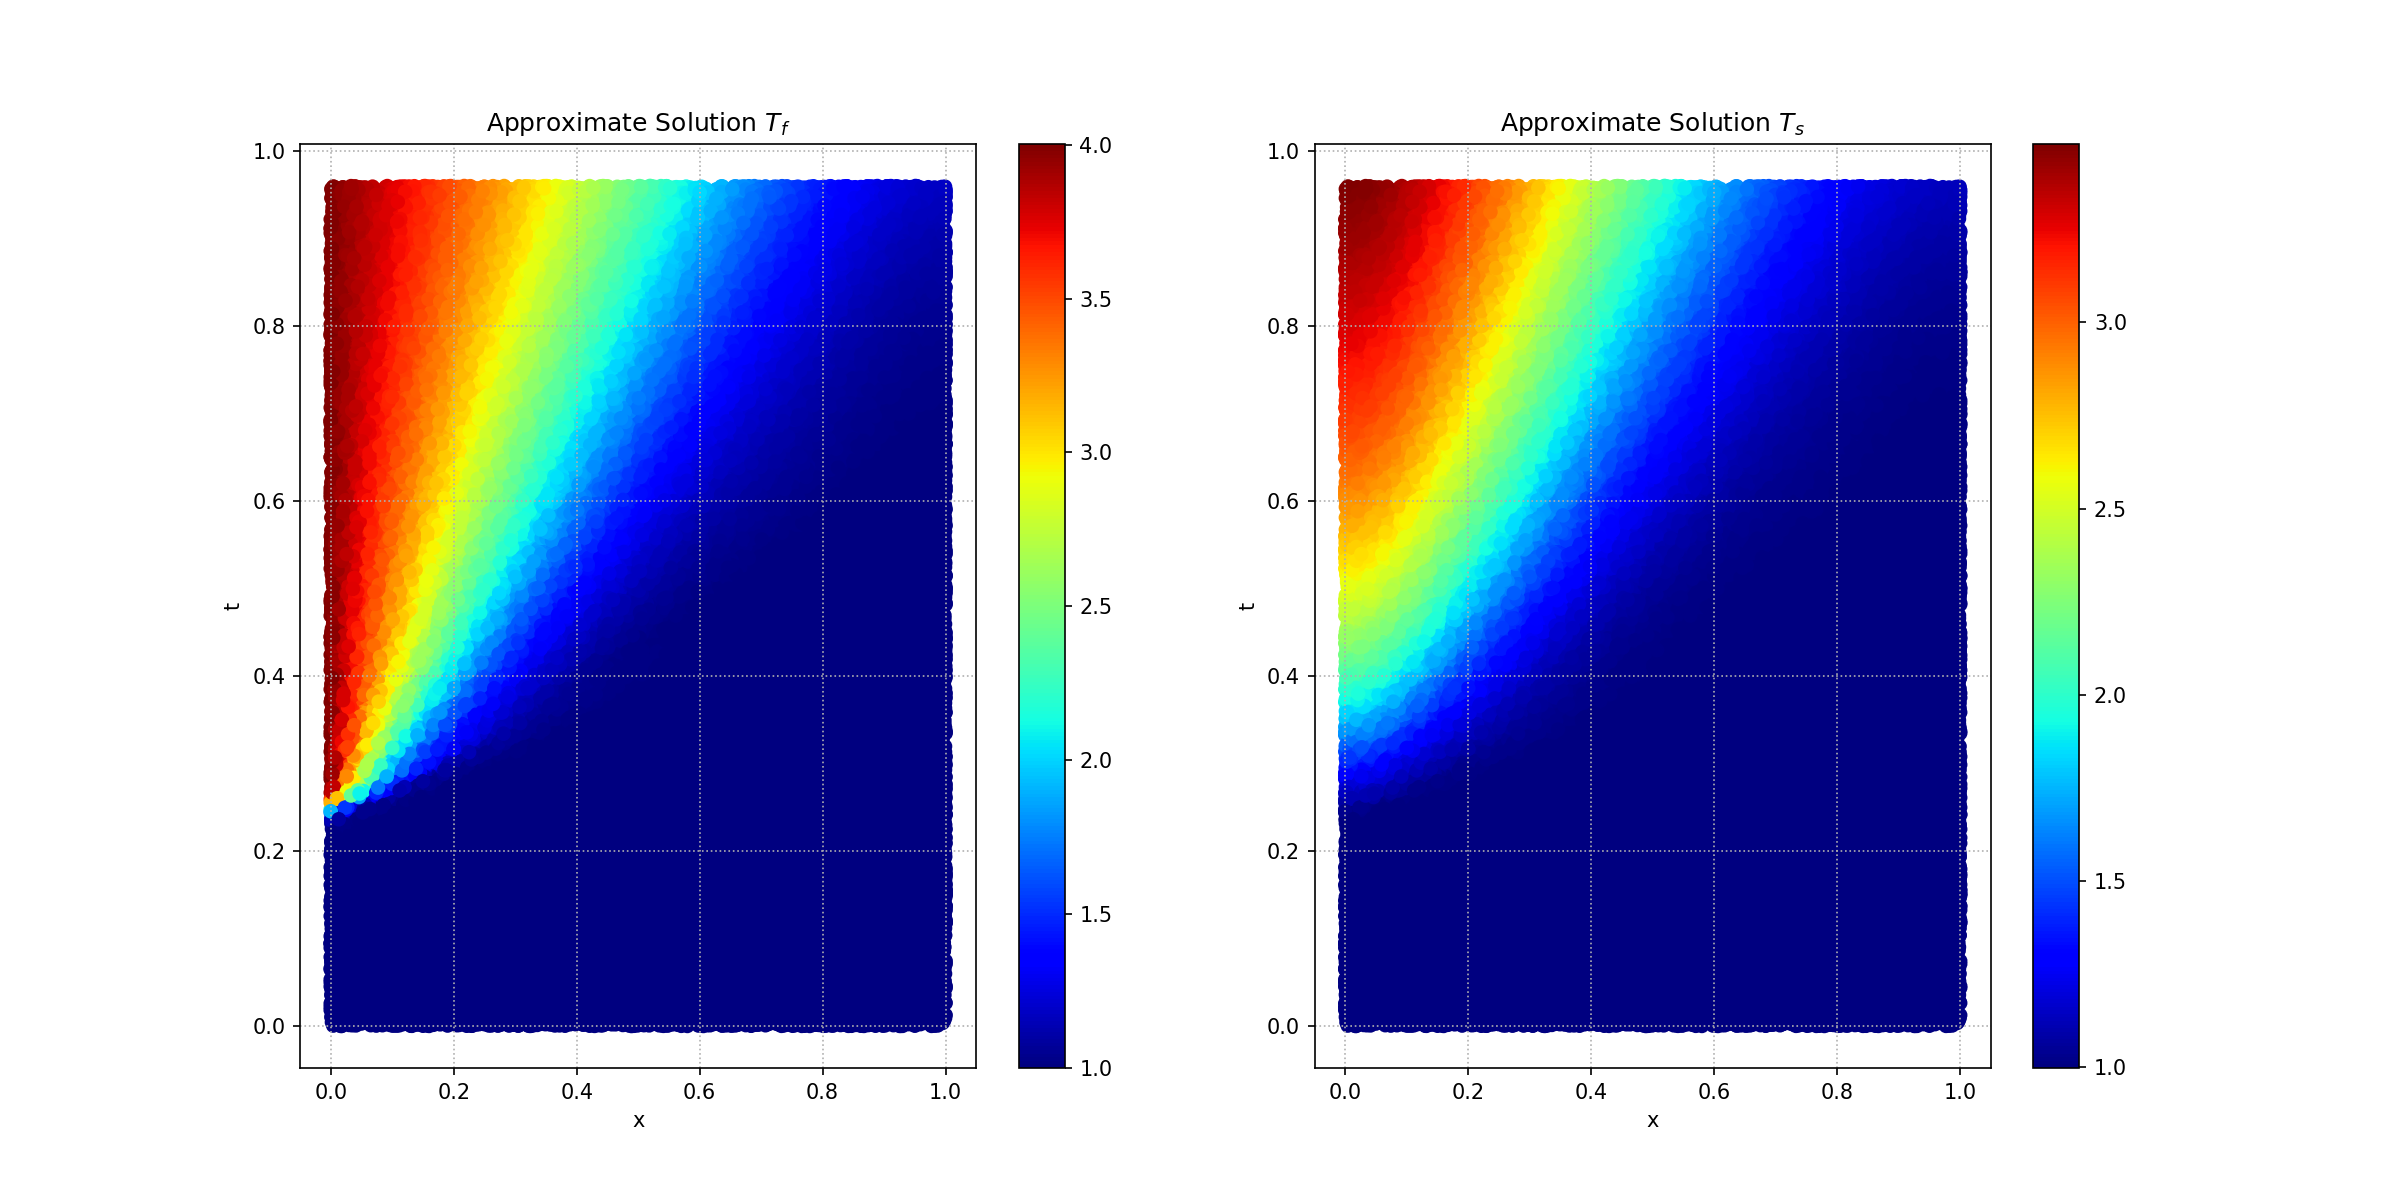
\includegraphics[width=.7\textwidth]{Graphics/Task1_Prediction_Solution.png}
    \caption{Predictions based on the trained PINN and test data as input.}
\end{figure}
\FloatBarrier


\section*{Task 2: PDE-Constrained Inverse Problem}
Consider now the equation governing the fluid temperature:
\begin{equation*}
\frac{\partial \bar{T}_{f}}{\partial t}(x, t)+U_{f}(t) \frac{\partial \bar{T}_{f}}{\partial x}(x, t)=\alpha_{f} \frac{\partial^{2} \bar{T}_{f}}{\partial x^{2}}-h_{f}\left(\bar{T}_{f}(x, t)-\bar{T}_{s}(x, t)\right) \quad x \in[0,1], t \in[0,8].
\end{equation*}
The goal of the task is to infer the values for the solid temperature $\bar{T}_{s}=\bar{T}_{s}(x, t)$, given input data of exact values of the fluid temperature $\bar{T}_{f}$ in the space-time domain using inverse algorithms.
The task has been solved using a PINN-algorithm using $2$ neural networks $\bar{T}_{f}^{\theta}$, $\bar{T}_{s}^{\theta}$ trained based on Sobol-points in the space-time domain. We used the  \textit{PINNs for Inverse Problems} as template for our implementation.
The following procedures in the template have been modified:
\begin{enumerate}
	\setlength\itemsep{-0.2em}
	\item\textit{add\_temporal\_boundary\_points}
	\item\textit{add\_spatial\_boundary\_points}
	\item\textit{add\_interior\_points}
	\item\textit{get\_measurement\_data}
	\item\textit{assemble\_datasets}
	\item\textit{apply\_boundary\_conditions}
	\item\textit{compute\_pde\_residual}
	\item\textit{compute\_loss}
\end{enumerate}



In this inverse problem the time horizon consists of $2$ cycles of lenght $T_{c}=4$. Each cycle consists of a \textit{charging phase}, an \textit{idle phase}, a \textit{discharging phase} and again an \textit{idle phase} each of lenght $1$.
Depending on the phase, the velocity of the fluid $U_{f}$ takes values in $\{1,0,-1\}$. This has been implemented in the procedure \textit{get\_fluid\_velocity}.
The boundary conditions for the fluid equation depend on the phase as well. This has been taken into account in the procedures \textit{add\_temporal\_boundary\_points} and \textit{apply\_boundary\_conditions}. The loss function defined in \textit{compute\_pde\_residual} forces the neural networks $(\bar{T}_{f}^{\theta}, \bar{T}_{s}^{\theta})$ to approximately satisfy the equation above for the fluid temperature
in the interior points which are again given by Sobol points as training data. This then allows us to infer values for the solid temperature $\bar{T}_{s}$ after training the networks. The loss function on \textit{compute\_loss} contains the usual loss for the fluid temperature $\bar{T}_{f}$ at the temporal and spatial boundary points. 

\begin{figure}[!htb]
    \centering
    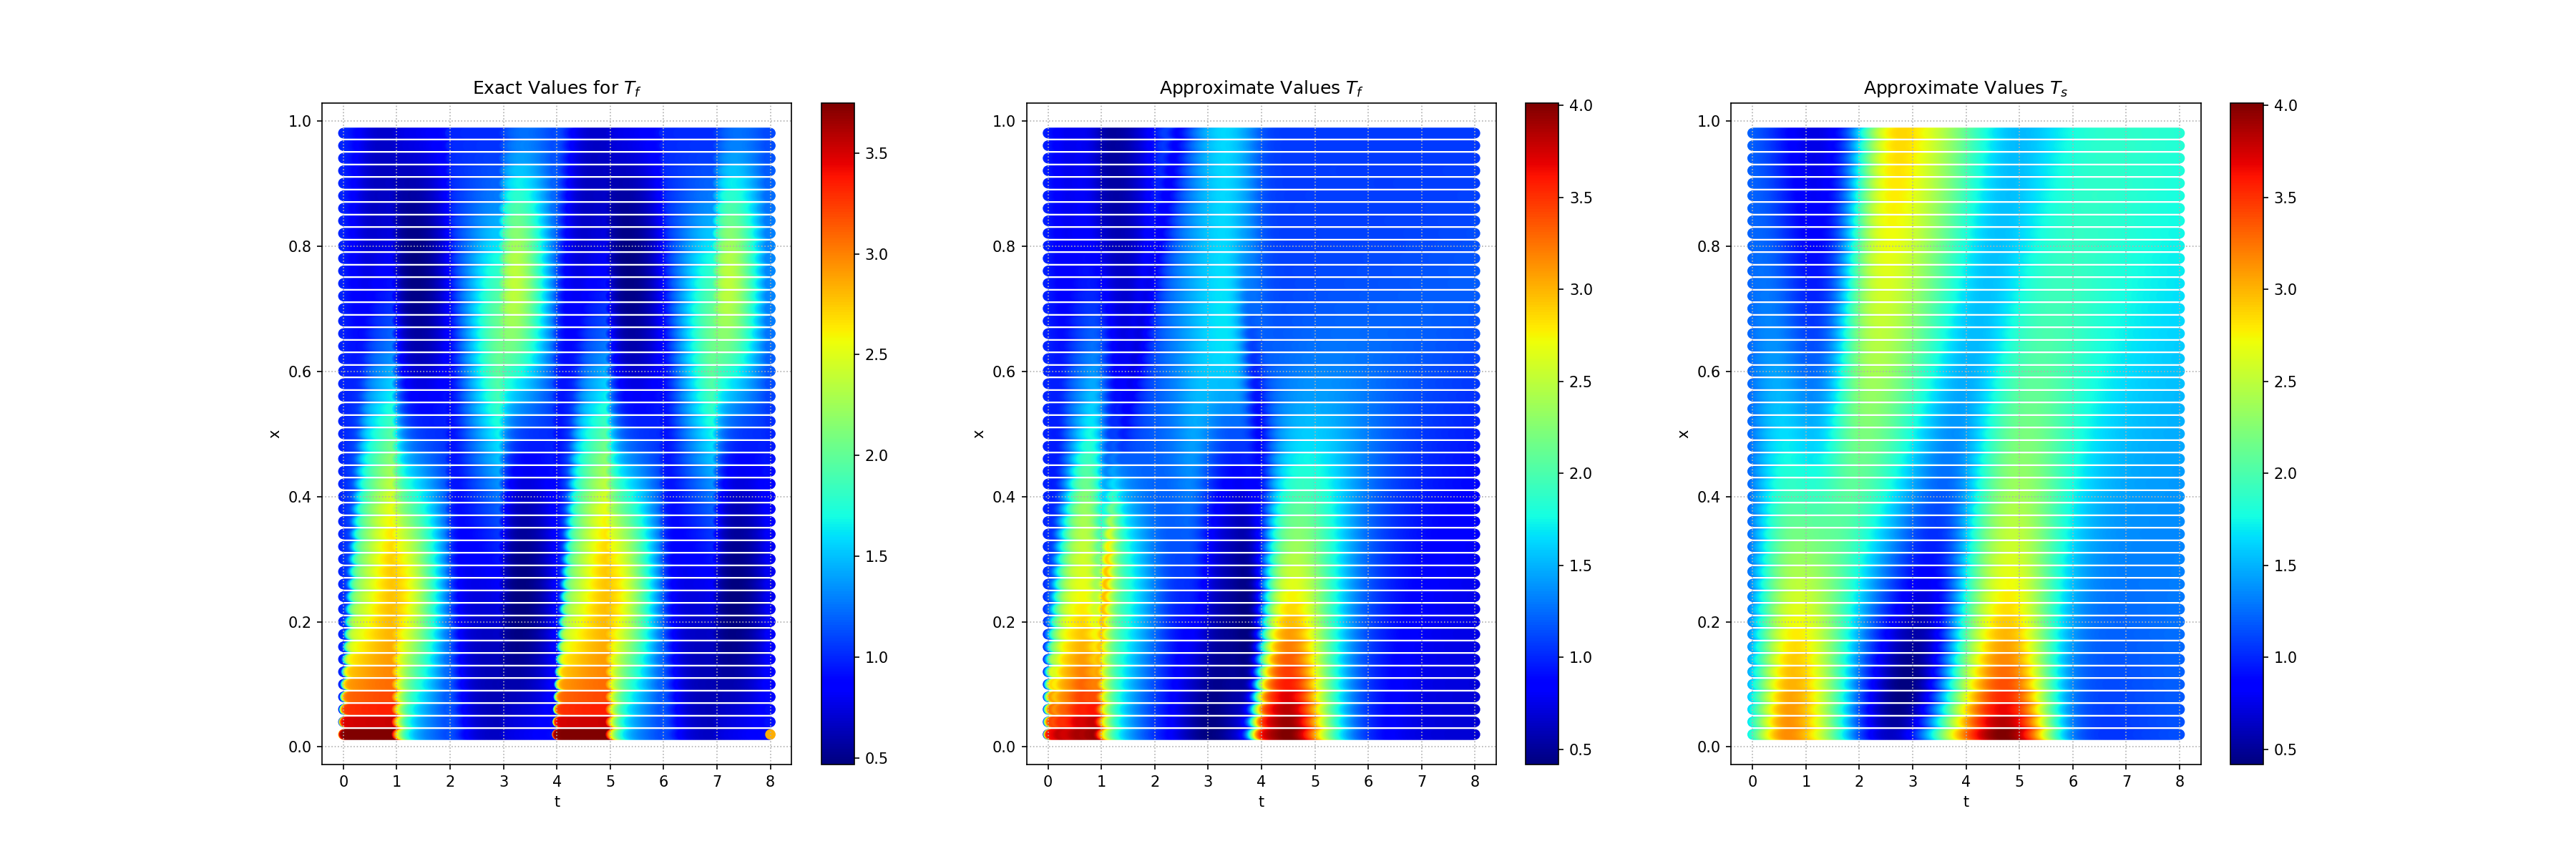
\includegraphics[width=.9\textwidth]{Graphics/Task2_Exact_Approximate_Solution.png}
    \caption{Exact values for $T_f$ beased on measurement data and predictions based on the trained PINN for $T_f$,  $T_s$.}
\end{figure}
\FloatBarrier




\section*{Task 3: Applied Regression}
Neural networks for regression tasks have been implemented in PyTorch on the dataset \textit{California Housing Data (1990)}. The dataset contains various features related to sociodemographic statistics such as \textit{medianIncome}, \textit{totalBedrooms}, \textit{population}. The goal is to predict the target variable \textit{median\_house\_value} based on the feature variables as input.

Various data transformations (feature scalings) have been examined on the input data to accomplish this task:
\begin{enumerate}
	\setlength\itemsep{-0.2em}
	\item Scaling down feature variable
  	\item Standardizing/normalizing input data
	\item Log-transforming input data
	\item Removing highly correlated input data
\end{enumerate}
To allow to examine the accuracy of our prediction on new data, the dataset has been split into training and testing data. The distribution of the numerical features have been studied. To remove skewed data (which might reduce the effect of outliers on the regression), it has been attempted as well
to log-transform the input data, which however led to poor prediction results. Correlations of the numerical features has been studied as well. To remove the effect of dimensionality and avoid overfitting, a naive approach has been used by removing highly correlated feature variables.

The targer variable has been scaled down by a factor of $100000$, which has been advantageous in terms of learning the neural networks.

For the log-transformed input data, a fully connected neural network with tunable parameters (amount of hidden layers, neurons per layer) with a single output-layer for the target variable and with a \textit{tanh}-activation for the hidden layers has been implemented. However the prediction based on the log-transformed input data led to rather poor prediciton results on the test data.

For the standardized input data, a fully connected neural network has been implemented as well. However here we used a \textit{ReLU}-activation for the hidden layers and for the final output-layer. The \textit{ReLU}-activation on the output-layer prevents negative predictions for the target variable.

Various parameters for the neural network have been tried out. It is found that many hidden layers and neurons lead to rather poor prediciton results on the test data, which is due to overfitting on the training data. A satisfying neural network was given by a very simple architecture: A single hidden layer with $2$ neurons. The calculated \textit{MSE} on test data and on the scaled target variable has been $0.5894$ which is comparable (but slightly above) other reference results on the same dataset.


\section*{Task 4: Robustness of PINNs and Transferability}
Consider the linear elliptic PDE given as differential operator:

\begin{equation*}
L_{f}u(x)\coloneqq\nabla (A(x) \nabla u(x)) - f(x) \text { for }x\in B_{1} \text { and }u \in C^{2}\left(B^{1}\right).
\end{equation*}

The matrix $A$ satisfies the usual ellipticity condition and $f\in L^{\infty}\left(B_{1}\right)$.

Set $f_{\delta}\coloneqq f+\delta \varphi$ for $\delta>0$ and $\varphi\in C^{\infty}_\text{Comp}$ such that $\varphi \leq 1$. Assume $u, u_{\delta} \in C^{2}\left(B^{1}\right)$ are solutions of $L_{f}$, $L_{f_\delta}$ respectively (I.e. $L_{f}u=0$, $L_{f_\delta}u_\delta=0$). 
By Linearity of the PDE, $u-u_{\delta}\in C^{2}\left(B^{1}\right)$ is a solution of $L_{f-f_\delta}$.
Hence applying the Schauder estimate and noticing that $\varphi \leq 1$ and $f-f_\delta = \delta \varphi$ we get the following inequality:

\begin{equation*}
\|u-u_{\delta}\|_{C^{1}\left(B_{1 / 2}\right)} \leq C\left(\|u-u_{\delta}\|_{L^{\infty}\left(B_{1}\right)}+\delta\right)
\end{equation*}

Assume we have a PINN-approximation $u_{\theta}\coloneqq N\!N_{\theta}(u)$ such that
$\left\|u_{\theta}-u\right\|_{C^{1}\left(B_{1}\right)} \leq \epsilon$ for some $\epsilon>0$.

Hence applying the triangle inequality and using the inequality above, we get the following estimate:

\begin{equation*}
\|u_{\theta}-u_{\delta}\|_{C^{1}\left(B_{1 / 2}\right)} \leq\epsilon + C\left(\|u-u_{\delta}\|_{L^{\infty}\left(B_{1}\right)}+\delta\right)
\end{equation*} 

Notice that the differential operator is continuous (it is enough to prove it for $L_0$, for which it follows from linearity and boundedness). The continuity and the estimate above have the following consequences when we let $\delta>0$ approach $0$:
\begin{itemize}
  	\item The gradient of the PINN-approximation is bounded, which is an advantage in terms of learning and for minimizing loss functions.
	\item  By continuity, we can choose $\delta>0$ small enough such that e.g. 
		$\|u_{\theta}-u_{\delta}\|_{C^{1}\left(B_{1 / 2}\right)} \leq 2\epsilon.$ Hence the PINN-approximation is robust w.r.t. perturbations.
\end{itemize}

The previous consideration leads us to propose the following \textit{transfer learning algoritm}:
\begin{enumerate}
	\setlength\itemsep{-0.2em}
	\item	Set $\delta>0$ as small as possible.
  	\item	Train a PINN for $u_{\delta}$.
\end{enumerate}

By setting  $\delta>0$ as small as possible the trained PINN-approximation is an approximation for $u$ as well, which follows from the robustness property discussed above.


\begin{thebibliography}{99}

\bibitem{BishopDL}
C. Bishop and H. Bishop, \textit{Deep Learning: Foundations and Concepts},\\
Springer, Switzerland, 2024.

\bibitem{CaliforniaHousing} \emph{California Housing Data (1990)},  available at\\
\texttt{https://www.kaggle.com/datasets/harrywang/housing}.

\bibitem{PytorchCaliforniaHousing} \emph{Regression with Neural Networks using PyTorch},  available at\\
\texttt{https://www.kaggle.com}.


\end{thebibliography}


\end{document}